\documentclass[conference]{IEEEtran}
\usepackage[utf8]{inputenc}
\usepackage[spanish]{babel}
\usepackage{graphicx}
\usepackage{amsmath}
\usepackage{float}
\usepackage{cite}

\begin{document}

\title{Informe de Laboratorio: Práctica 0 - Manejo de Equipos}

\author{\IEEEauthorblockN{Estudiante 1}
\IEEEauthorblockA{\textit{Departamento de Ingeniería Eléctrica y Electrónica} \\
\textit{Universidad Nacional de Colombia}\\
Bogotá, Colombia \\
correo1@unal.edu.co}
\and
\IEEEauthorblockN{Estudiante 2}
\IEEEauthorblockA{\textit{Departamento de Ingeniería Eléctrica y Electrónica} \\
\textit{Universidad Nacional de Colombia}\\
Bogotá, Colombia \\
correo2@unal.edu.co}
\and
\IEEEauthorblockN{Estudiante 3}
\IEEEauthorblockA{\textit{Departamento de Ingeniería Eléctrica y Electrónica} \\
\textit{Universidad Nacional de Colombia}\\
Bogotá, Colombia \\
correo3@unal.edu.co}
}

\maketitle

\begin{abstract}
El presente informe documenta el trabajo previo para la práctica de manejo de equipos de medición en el laboratorio de electrónica análoga. Se abordan los cálculos teóricos, simulaciones con sus respectivas formas de onda ilustrativas y conceptos fundamentales para el uso del generador de señales, osciloscopio y multímetro digital.
\end{abstract}

\section{Introducción y Justificación}
La correcta operación de los equipos de medición electrónica es un pilar fundamental en la ingeniería. Esta práctica busca desarrollar habilidades prácticas en la medición de voltaje, corriente, potencia y la caracterización de impedancias de entrada y salida de los instrumentos.

\textbf{Justificación y Aplicación en la Vida Real:}
El dominio de estos conceptos tiene aplicaciones directas en campos de alta exigencia tecnológica. Por ejemplo, en misiones espaciales de la NASA, la recolección de datos mediante telemetría y sensores depende de un riguroso acondicionamiento de señales. Si los ingenieros no calculan y acoplan correctamente las impedancias de entrada y salida entre los sensores de un satélite y sus sistemas de transmisión, se producen reflexiones de señal y atenuaciones críticas. Esto podría resultar en la pérdida de datos vitales sobre el estado de la nave o parámetros atmosféricos. El conocimiento de los valores RMS, niveles DC y la impedancia asegura que la instrumentación aeroespacial funcione de manera óptima y sin pérdidas de potencia.

\section{Cálculos y Trabajo Previo}

\subsection{Cálculos del Circuito Resistivo}
Para el circuito resistivo propuesto, se aplican las leyes de Kirchhoff para hallar los voltajes de nodo y posteriormente corrientes y potencias.

\begin{itemize}
    \item $V_1 = 5$ V.
    \item $R_1 = 1$ k$\Omega$, $R_2 = 2.2$ k$\Omega$, $R_3 = 2.2$ k$\Omega$, $R_4 = 1$ k$\Omega$.
\end{itemize}

Resolviendo el sistema de ecuaciones para los nodos principales, se obtienen teóricamente los siguientes valores de voltaje:
$V_{N2} \approx 2.83$ V y $V_{N3} \approx 0.88$ V. 
Las corrientes y potencias se calculan mediante la Ley de Ohm ($I = V/R$) y la ecuación de potencia ($P = V \cdot I$).

\subsection{Cálculos de Señales (Ecuaciones)}
Para encontrar el valor medio (DC) y el valor eficaz (RMS) de las señales solicitadas, se emplean las siguientes definiciones matemáticas \cite{sedra2020}:

Valor Medio (DC):
\begin{equation}
    V_{DC} = \frac{1}{T} \int_{0}^{T} v(t) dt
\end{equation}

Valor Eficaz (RMS):
\begin{equation}
    V_{RMS} = \sqrt{\frac{1}{T} \int_{0}^{T} v(t)^2 dt}
\end{equation}

\section{Simulaciones}
Se realizó la simulación del circuito resistivo y de las señales propuestas. En la Figura \ref{fig:circuito} se observa el esquema del circuito implementado.

\begin{figure}[H]
    \centering
    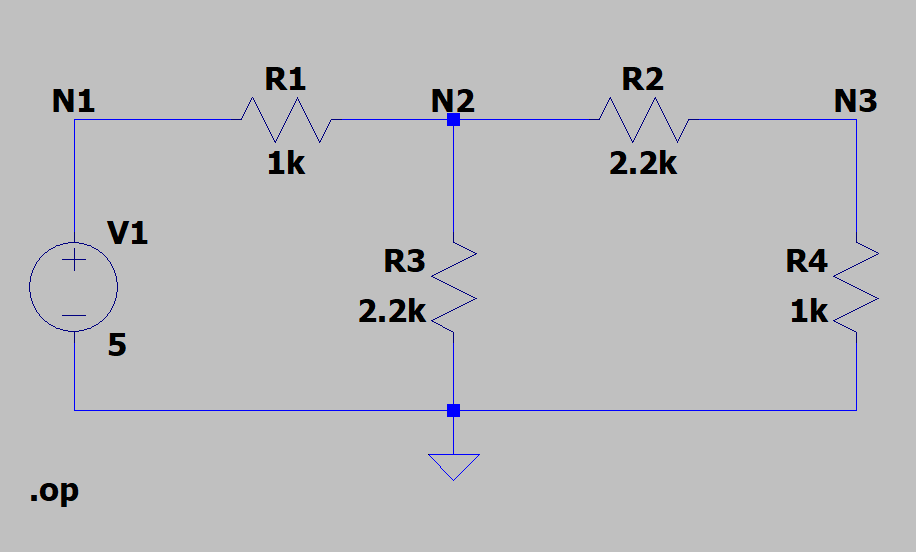
\includegraphics[width=0.45\textwidth]{analoga_practica1_3.1.2.png}
    \caption{Esquema del circuito resistivo propuesto.}
    \label{fig:circuito}
\end{figure}

El punto de operación (Operating Point) arrojado por el simulador se reporta en la Figura \ref{fig:op_point}.

\begin{figure}[H]
    \centering
    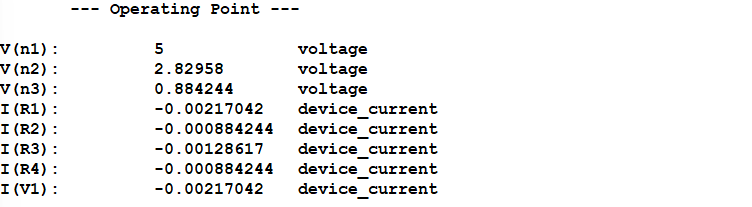
\includegraphics[width=0.45\textwidth]{analoga_grafica_sinoidal_2.png}
    \caption{Punto de operación simulado mostrando los voltajes y corrientes del circuito resistivo.}
    \label{fig:op_point}
\end{figure}

Para ilustrar de forma clara las formas de onda generadas y analizadas en el trabajo previo, las Figuras \ref{fig:sin_l}--\ref{fig:tri_l} muestran las 4 gráficas limpias obtenidas en la simulación:

\begin{figure}[H]
    \centering
    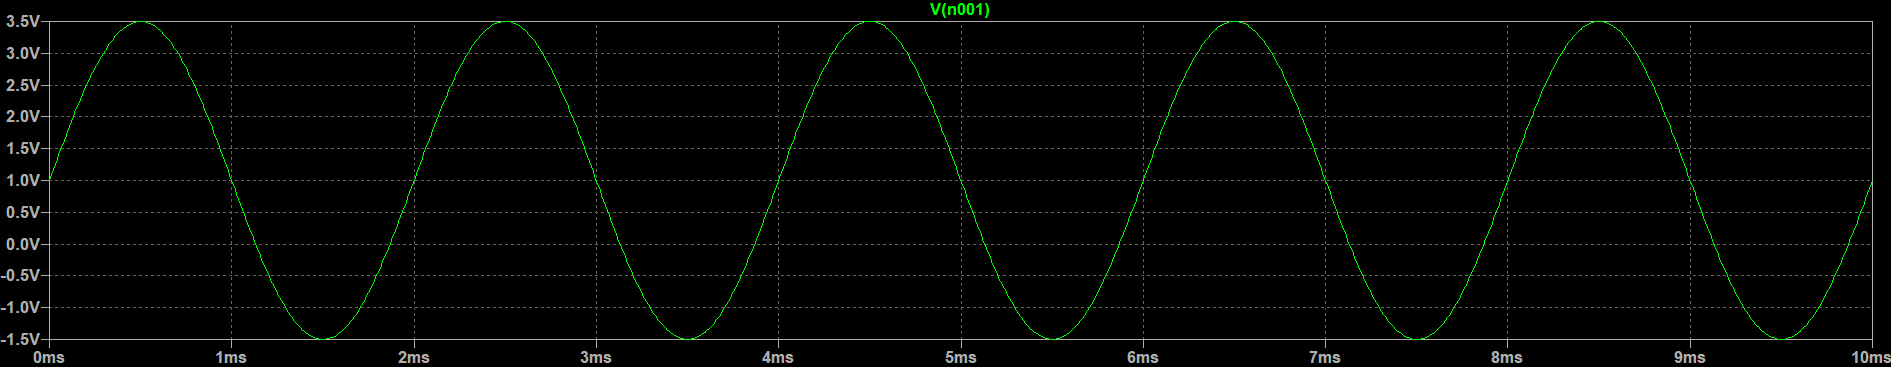
\includegraphics[width=0.45\textwidth]{analoga_grafica_sinoidal_1.png}
    \caption{Señal senoidal limpia simulada.}
    \label{fig:sin_l}
\end{figure}

\begin{figure}[H]
    \centering
    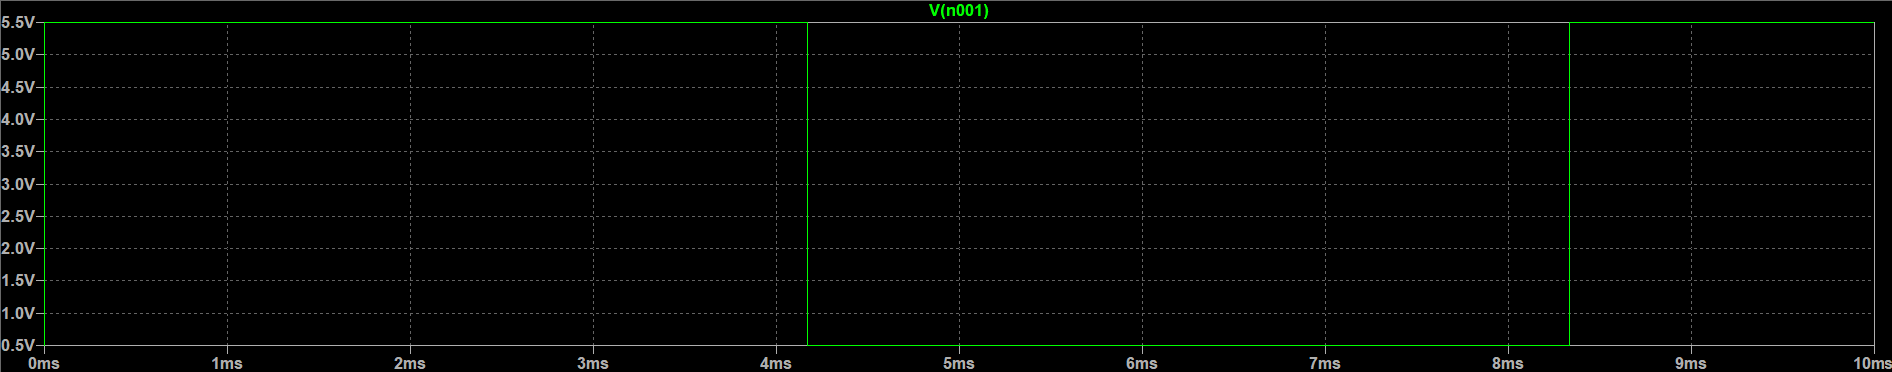
\includegraphics[width=0.45\textwidth]{analoga_grafica_cuadrada_1.png}
    \caption{Señal cuadrada limpia simulada.}
    \label{fig:cua_1_l}
\end{figure}

\begin{figure}[H]
    \centering
    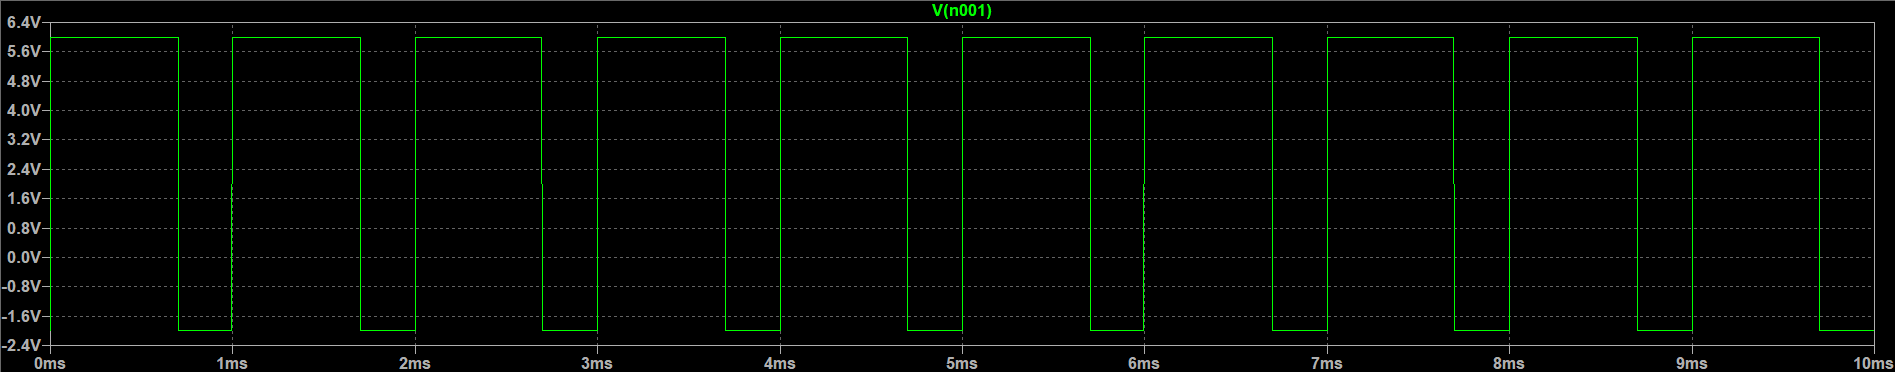
\includegraphics[width=0.45\textwidth]{analoga_grafica_cuadrada_2_1.png}
    \caption{Señal cuadrada simétrica limpia simulada.}
    \label{fig:cua_2_l}
\end{figure}

\begin{figure}[H]
    \centering
    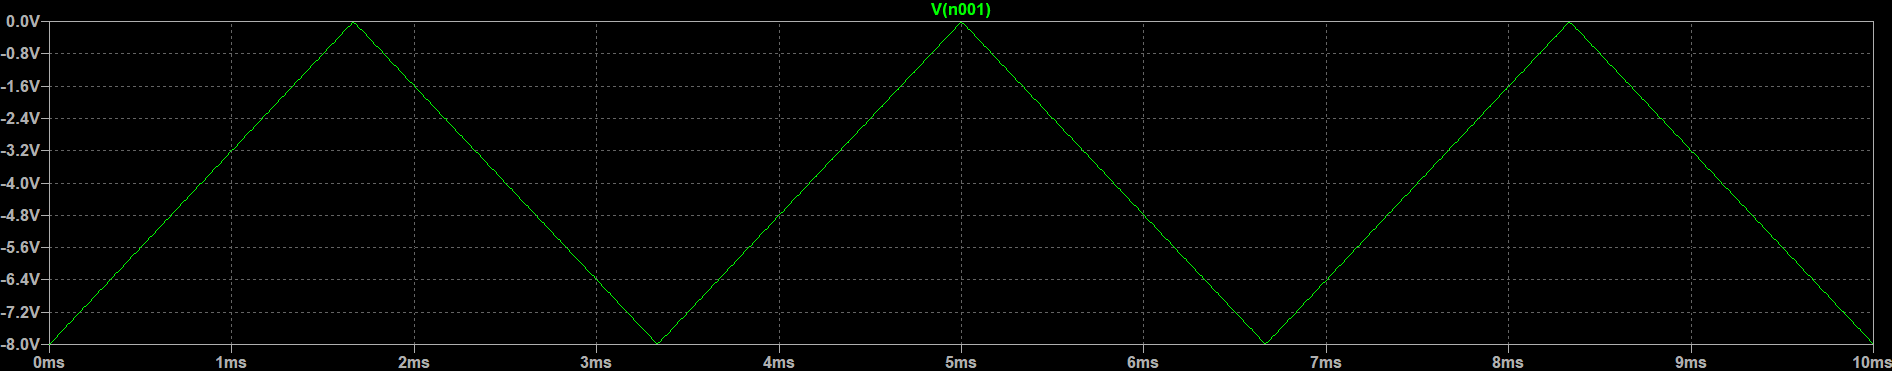
\includegraphics[width=0.45\textwidth]{analoga_grafica_triangular_1.png}
    \caption{Señal triangular limpia simulada.}
    \label{fig:tri_l}
\end{figure}

\section{Respuestas a las Preguntas Sugeridas}

\begin{enumerate}
    \item \textbf{¿Cómo es el proceso que realiza cada tipo de multímetro para completar su proceso de medición?} \\
    Un multímetro digital estándar realiza un muestreo de la señal mediante un Conversor Analógico a Digital (ADC). Para señales DC, promedia las muestras. Para señales AC, un multímetro convencional rectifica la señal y la multiplica por un factor de forma (asumiendo que es senoidal pura). Un multímetro \textit{True RMS} realiza el cálculo matemático real (raíz del promedio de los cuadrados) muestreando la señal de entrada, lo que permite medir ondas no senoidales con precisión.
    
    \item \textbf{¿Qué variables de las funciones generadas pueden ser medidas por cada dispositivo de medición?} \\
    El multímetro puede medir valores escalares como el voltaje eficaz (RMS), el voltaje medio (DC), la corriente y la frecuencia. El osciloscopio, al ser un instrumento gráfico, permite medir variables en el dominio del tiempo: amplitud (pico y pico a pico), periodo, frecuencia, fase, tiempos de subida/bajada, ciclo útil y visualizar la forma exacta de la onda.
    
    \item \textbf{¿Por qué los multímetros tienen un límite de frecuencia?} \\
    Debido a las limitaciones físicas de sus componentes internos, específicamente el ancho de banda de los amplificadores operacionales de entrada y la tasa de muestreo del conversor ADC. A altas frecuencias, la circuitería no logra seguir los cambios rápidos de la señal, atenuando la lectura.
    
    \item \textbf{¿Qué es la precisión vertical en un osciloscopio y de qué depende?} \\
    Es la capacidad del osciloscopio para resolver pequeños cambios en el voltaje de la señal. Depende principalmente de la resolución en bits de su Conversor Analógico a Digital (ADC) (típicamente de 8 a 12 bits) y del nivel de ruido del amplificador de entrada.
    
    \item \textbf{¿Qué significa impedancia de salida y de entrada?} \\
    La \textit{impedancia de salida} es la resistencia equivalente de Thevenin que presenta un equipo (como el generador) hacia la carga que se le conecta. La \textit{impedancia de entrada} es la resistencia equivalente que un equipo (como el osciloscopio) presenta a la fuente de señal. Conocerlas es vital para garantizar la máxima transferencia de potencia o evitar efectos de carga indeseados.
\end{enumerate}

\section{Montaje}
\textit{[Espacio reservado para documentar el montaje físico en protoboard una vez se realice la práctica en el laboratorio.]}

\vspace{2cm}

\section{Análisis de Resultados}
\textit{[Espacio reservado para contrastar los datos medidos con los equipos físicos frente a los cálculos y simulaciones.]}

\vspace{2cm}

\section{Conclusiones}
\textit{[Espacio reservado para las conclusiones finales basadas en la práctica de laboratorio.]}

\vspace{2cm}

\begin{thebibliography}{1}
\bibitem{sedra2020}
A. S. Sedra, K. C. Smith, T. C. Carusone, y V. Gaudet, \emph{Microelectronic Circuits}, 8va ed. New York, NY: Oxford University Press, 2020. ISBN 9780190853464. Copyright \copyright 2020 by Oxford University Press.
\end{thebibliography}

\end{document}